\documentclass[12pt]{article}
%\documentclass[10pt, landscape, twocolumn]{article}

%\usepackage{setspace}
%\onehalfspacing
\usepackage[T2A]{fontenc}
\usepackage[utf8]{inputenc}

\usepackage[russian]{babel}

\usepackage{amsmath, amssymb}
%\usepackage[lastpage,user]{zref}

\usepackage{geometry, graphics, graphicx}

\graphicspath{ {./images/} }

\geometry
{
    a4paper,
    total={210mm,297mm},
    left=20mm,
    right=20mm,
    top=25mm,
    bottom=20mm,
}

\usepackage{hyperref}

\hypersetup{
    colorlinks=false,       % false: boxed links; true: colored links
    linkcolor=red,          % color of internal links (change box color with linkbordercolor)
    citecolor=green,        % color of links to bibliography
    filecolor=magenta,      % color of file links
    urlcolor=cyan           % color of external links
}

% ------------Колонтитулы-----------------
%\usepackage{fancyhdr}
%\pagestyle{fancy}
%
%\fancyhead{}
%\lhead{}
%\chead{}
%\rhead{}
%\lfoot{\scriptsize\textbf{UPD.:}~\emph{\today}}
%\cfoot{}
%\rfoot{\thepage /\zpageref{LastPage}}


%\usepackage{amsopn}
%\DeclareMathOperator{\B}{B}

\usepackage{hyperref}


%\usepackage{tikz}
%\usepackage{background}
%\usepackage{tikzpagenodes}
%\usepackage{lmodern}
\usepackage{indentfirst}

%\backgroundsetup%
%{   angle=0,
%    opacity=2,
%    scale=1,
%    contents=%
%    {   \begin{tikzpicture}[remember picture,scale=3]
%            \fontsize{100}{120}\selectfont
%            \node[text=gray!50,rotate=90, above=1cm] 	at (current page text area.west) {\textbf{ФН--1}};
%            \node[text=gray!50,rotate=-90, above=1cm] 	at (current page text area.east) {\textbf{ФН--1}};          
%        \end{tikzpicture}
%    }
%}
% ----------------------------------------

%\newcommand{\ul}{\underline}

%\usepackage{amsopn}
%\DeclareMathOperator{\up}{up}
%\DeclareMathOperator{\h}{h}
%\DeclareMathOperator{\fup}{fup}
%%\DeclareMathOperator{\ch}{ch}
%\DeclareMathOperator{\g}{g}

\usepackage{xcolor}
\definecolor{amaranth}{rgb}{0.9, 0.17, 0.31}
\definecolor{amethyst}{rgb}{0.6, 0.4, 0.8}
\definecolor{ao}{rgb}{0.0, 0.0, 1.0}


\title{Применение свёрточных нейронных сетей в задаче оптического распознавания текста для фильтрации нежелательных данных}
\author{Разумов Т.Е., Чуриков Д.В., Кравченко О.В.}

\begin {document}
\maketitle

\begin{abstract}
В настоящей работе решается задача построения модели для обнаружения и фильтрации нежелательных спам--сообщений. В качестве модели классификатора нежелательных писем в электронной почте выбрана полносвязная свёрточная нейронная сеть (\textsf{FCNN}). Она позволяет разделить письма на две категории: \emph{спам} и \emph{не спам}. 

Основным результатом исследования является программное приложение на языке \textsf{C++}, имеющее микро--сервисную архитектуру, и решающее задачу классификации изображений. Приложение способно выдерживать более $10^6$ запросов в минуту в режиме реального времени.
\end{abstract}


\section{Введение}
Currently, the amount of information produced by humanity
is increasing exponentially. Significant benefits can be derived from this information only if the data is properly processed and analyzed.

On the other hand, the actual task of data processing is the task
of filtering unwanted data, and in relation to IT technologies --- this is the task of filtering spam messages.
The latter is due to the fact that the exchange of information of various information by default uses email. Email is one of the cheapest, easiest to use, most easily accessible, most official, and most reliable ways to exchange information.

Spam-messages, in general, may contain heterogeneous test-visual information. Deep
learning algorithms are used to analyze spam emails with various information received in real time in \cite{Makkar2021}.
At the same time, the features (characteristics) are first extracted from the image),
and then the decision is made.


Other classification approaches include the support vector machine and the random forest method. The paper \cite{Taylor2020} compares these methods for solving the problem of filtering spam messages.

Filtering algorithms are usually stochastic \cite{Garg2021}
and are used in combination with optimization methods for some objective function.
Various probabilistic models are used to solve the problem of email classification. The most commonly used among them is the naive Bayesian classifier. The particle swarm method is one of the numerical methods of stochastic optimization, it is used in data filtering problems, since it is not necessary to specify an analytical expression of the gradient of the optimized function.
The particle swarm method refers to stochastic optimization methods and is used for heuristic global optimization of the parameters of a naive Bayesian classifier. A complex approach using the naive Bayes algorithm together with the particle swarm optimization method was applied in \cite{Parmar2020}.
The evolutionary model of spam classification is presented in \cite{Mohammad2020}.

{
\bf\color{amaranth}
Добавить абзацы про задачу и её решение настоящей статьи.
}



\section{Методология}
\subsection{Формальная постановка задачи}
Пусть задано некоторое множество объектов $ X = X_L \cup X_T $, где 
$X_L$ --- обучающая выборка, 
$X_T$ --- тестовая выборка, 
$Y$ --- множество допустимых ответов. Считаем, что существует некоторая целевая функция $g: X \rightarrow Y$, значения которой известны только на множестве $X_L$. Пусть данные распределены в соответствии с некоторым неизвестным распределением $P(x,y) = P(x) P(y|x)$, при этом задана некоторая функция потерь
$$
R(g(x), y) = 
\begin{cases} 
\phantom{>}0, & y = g(x), \\
> 0, & y \neq g(x).
\end{cases}
$$

В соответствии с принципом минимизации эмпирического риска 
{\bf\color{amaranth} (что за принцип?)} нам надо минимизировать функцию потерь, то есть найти такую решающую функцию $g(x)$, которая в среднем будет приводить к наименьшей погрешности. Формально, требуется решить следующую задачу минимизации
$$
g(x) = \operatorname*{argmin}_{f: X \rightarrow Y} E_{X,Y} R(f(x), y).
$$

Для задачи фильтрации нежелательных данных множество $Y$ состоит из двух элементов $\{0, 1\}$, где $0$ и $1$ желательные и нежелательные данные соответственно. В силу грубости методов дискретных вычислений, на практике обычно используется $Y = R[0, 1]$, а результат работы классификатора $y' = g(x)$ {\bf\color{amaranth} (почему стоит штрих?)} отноcится к нужному классу с заданной пороговой вероятностью $\alpha$, минимизирующей ошибку первого и второго рода.

\subsection{Требования к решению}
Currently, information is moving at a high speed, which imposes an additional important requirement on the speed of the model and the system as a whole. The time for checking a single message should not exceed $\leqslant3$ seconds, which imposes additional requirements on the tools used and the fault tolerance of the entire system.

\section{Методология}

From the moment of receiving the message to the moment of making a decision about its type, the text information goes through several stages of processing:
\begin{enumerate}
\item Preprocessing.
\item Vectorization.
\item Classification.
\end{enumerate}

\subsection{Предобработка текста}
Since the text has a very heterogeneous structure and a single word can be written in many different ways (different font, encoding, case, etc.), but still have the same meaning, different methods of preprocessing the text or a combination of them are used.

The first step is to parse the text and decode it into the specified encoding. Then the conversion to the lower (or upper) case, removing unnecessary spaces, indents. The characters are replaced according to the specified rule. After that, the following methods are applied:

\subsubsection*{\it\,Stop words}
The text often contains many characters that do not carry a semantic load for the general meaning (two spaces, paragraph indentation), as well as stop words.
Stop words are words in any language that don't add much meaning to a sentence. Often, stop words include punctuation marks, pronouns, and prepositions. Often, spammers use them to make texts noisy in order to hide the spam content of the message. Since they can be safely ignored without sacrificing the meaning of the sentence, classification tasks often resort to removing them from the original message.

\subsubsection{\it\,Стемминг и лемматизация}
Обычно тексты содержат разные грамматические формы одного и того же слова, а также могут встречаться однокоренные слова. Используя разные алгоритмы лемматизация и стемминг преследуют цель привести все встречающиеся словоформы к одной, нормальной словарной форме.


Стемминг -- это грубый эвристический процесс, который отрезает "лишнее" от корня слов, часто это приводит к потере словообразовательных суффиксов. Основная проблема, возникающая при использовании стеммера -- это обработка слов, которые при образовании разных грамматических форм меняют не только окончание, но и основу слова. Например, существительное "кошка" в винительном и родительном падеже множественного числа имеет форму "кошек". Из-за таких беглых гласных стеммер должен либо игнорировать подобные формы, усекая "кошки" до "кошк" и теряя часть форм слова, либо усекать слово до безусловно неизменяющейся основы, получая "кош", что впоследствии может привести к полной потере контекста. Чтобы минимизировать негативные последствия слишком агрессивного усечения слов стеммером, необходимо выполнять стемминг искомого ключевого слова, а затем сравнивать результат с выходом стеммера для каждого из слов в обрабатываемом тексте. Но даже в этом случае буду встречаться совпадения стемов для совершенно несвязанных слов.


Лемматизация -- это более тонкий процесс, который использует словарь и морфологический анализ, чтобы в итоге привести слово к его канонической форме (лемме). Однако он применяет упрощенный анализ слов, не учитывая контекст. Это приводит к неоднозначностям при определении части речи. Например, лемматизация слов в словосочетании "мы роем яму" даст для второго слова два варианта лемматизации: существительное рой и глагол рыть. Эта неоднозначность не может быть разрешена без привлечения морфологического анализатора.

Как правило лемматизация дает наиболее точные результаты и именно этот подход используется в работе.

\subsection{Векторизация текста}
Modern machine learning algorithms cannot directly work with raw text, so it is necessary to build a text mapping to a vector space. This is called feature extraction. Let's consider several approaches for constructing this mapping.

\subsubsection*{\it\,Мешок слов}
Модель "мешок слов" - это упрощенное представления текстовой информации, используемое в задачах обработки естественных языков и поиска информации. В этой модели текст представляется в виде мешка (мультимножества) его слов или словосочетаний в случае комбинаций термов, игнорируя грамматику и в некоторых случаях даже порядок слов, но сохраняя множественность. Каждому такому терму (слову или словосочетанию) ставится в соответствие некоторое число. В этом случае текст определяется вектором $x=(x_1, ..., x_N)^T$, где $N$ - размерность из конечного словаря $X_L$ состоящего из уникальных термов обучающей выборки. Возможны следующие варинаты определения $x_i$
\begin{itemize}
\item Булевский вес: $\begin{cases} 1, & \mbox{если элемент присутствует в письме} \\ 0, & \mbox{если элемент не присутствует в письме}  \end{cases}$
\item Количество вхождений i-го терма в тексте: $x_i = n_i$
\item Частота терма: $x_i = \dfrac{n_i}{\sum n_k}$
\end{itemize}

В данной работе для определения $x_i$ мы взяли частоту терма.

\subsubsection*{\it\,Word2Vec}

The main problem with BOW is the loss of context between words. Since in natural language, the permutation of even two words of a sentence can completely change its meaning, this classification approach may have low accuracy.

Word2Vec is a text vectorization tool that takes into account the contextual relationship between words. The algorithm is based on such methods as huffman binary tree, skip-gram, negative sampling. The main problem with Word2Vec is finding the context for rare words.

\subsubsection*{\it\,Fast Text}

FastText --- is a Word2Vec extension proposed by Facebook in 2016. Instead of entering individual words into a neural network, Fast Text splits the words into several n-grams (proverbs). For example, the trigrams for the word "apple" --- are "app", "ppl", and "pll" (excluding the beginning and end of word boundaries). The vector for the word "apple" is formed by the sum of all n-grams. After training the neural network, we will have embedding words for all n-grams from the training dataset.

With this approach, the algorithm becomes more sensitive to rare words, since it is very likely that some of their n-grams are also present in other words. It takes longer to train the Fastext model, but it works better than Word2Vec and allows you to correctly represent rare words.

\subsection*{Классификация текста}
После векторизации текста мы должны построить преобразование из множества признаков во множество классифицируемых объектов $g: X \rightarrow Y$ 

Согласно статье [twitter threshold p. 4.6] была произведена разметка уникальных точек по бинам и вычеслена оптимальная пороговая точность $\alpha = 0.75$, которая обеспечивает оптимальный pressision и recall для нашей модели и минимизует дисперсию ошибки.

\subsubsection*{\it\,Логистическая регрессия}
Наиболее частым методом используемым в задаче классификации используется метод логистической регрессии:
$$
g(x) = \left(1 + \exp{ \left( \sum_{i=0}^n w_i x_i  \right) }\right)^{-1},
$$
где $w=(w_1, ..., w_N)^T$ --- веса модели, полученные при обучении.

Приведем результаты расчетов для разных способов векторизации текста.

Для BOW эмбедингов мы имеем следующие результаты:
\begin{center}
  \begin{tabular}{ | c | c |}
    \hline
     precision & recall \\ \hline
     0.91143 & 0.99961 \\ \hline
  \end{tabular}
\end{center}


Для Fast Text эмбедингов мы имеем следующие результаты:
\begin{center}
  \begin{tabular}{ | c | c |}
    \hline
     precision & recall \\ \hline
     0.95523 & 0.89164  \\ \hline
  \end{tabular}
\end{center}

\subsubsection*{\it\,Fully convolutional neural network}

Fully convolutional neural network для нашей задачи имеет 3 слоя. На первых двух используется функция активации $ReLU$, на последнем $Sigmoid$. На каждом слое производится регуляризация данных. В нашем случае нейронную сеть можно определить формулой:

$$
g(x) = h_2 \left(\sum_{k=0}^{n_2} w''_k h_1\left(\sum_{j=0}^{n_1} w'_j h_0\left( \sum_{i=0}^{n_0} w_i x_i \right)\right)\right),
$$

где $h_i$ -- функция активации для соответствующего слоя. Для нахождения весов $\{w_i\}$, $\{w'_j\}$, $\{w''_k\}$ на этапе обучения модели используется метод Адама.

Для BOW эмбедингов мы имеем следующие результаты:
\begin{center}
  \begin{tabular}{ | c | c |}
    \hline
     precision & recall \\ \hline
     0.93604 & 0.95643 \\ \hline
  \end{tabular}
\end{center}

Для Fast Text эмбедингов мы имеем следующие результаты:
\begin{center}
  \begin{tabular}{ | c | c |}
    \hline
     precision & recall \\ \hline
     0.99931 & 0.91263 \\ \hline
  \end{tabular}
\end{center}

\subsection{Аспекты реализации алгоритмов}

\subsubsection*{\it\,Микросервисная архитектура}

Since the service must operate under high loads, it is important to provide an architecture in which the failure of one component does not lead to the degradation of the entire system. The following client-server architecture is implemented (Fig. 1). Antispam daemon (mrasd) parses incoming messages and extracts text, images, and files from there. Since unwanted data is often contained inside nested images and documents, it is also necessary to extract text from them. To do this, the documents are sent to the OCR service via a deferred redis queue, which extracts the text and stores the result in the redis cache.

Since, with a high probability, the letter can be a duplicate (for example, in the case of a ddos attack or offline rechecking), in order not to load the OCR service once again, the primary check of the redis cache is performed for the presence of already processed data for the specified document hash.

After full text extraction, the mrasd service performs all the steps of text preprocessing (reduction to a single register, removal of stop words, normalization), and then sends the text to the mlapi service via the grpc protocol to vectorize the text using fast text and further obtain the fcnn prediction of the model by which a decision is made about the" undesirability " of the incoming message.

The proposed architecture is good because when the OCR of seris, one (or several) instances of redis cluster fails, the entire system as a whole does not degrade.
 
\begin{figure}[h!]
	\center
	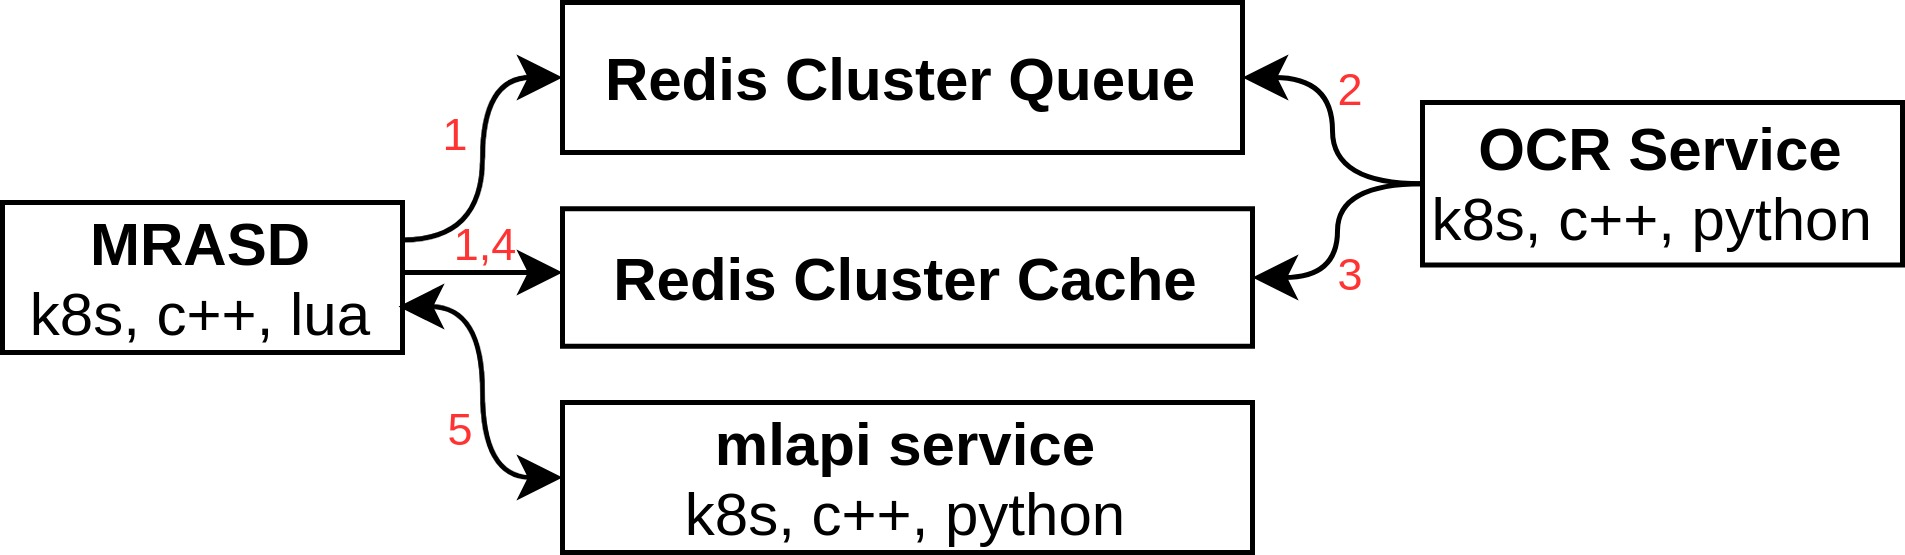
\includegraphics[scale=0.25]{deploy.jpg}
	\caption{Deploy}
	\label{fig:02}
\end{figure}


\begin{figure}[h!]
	\center
	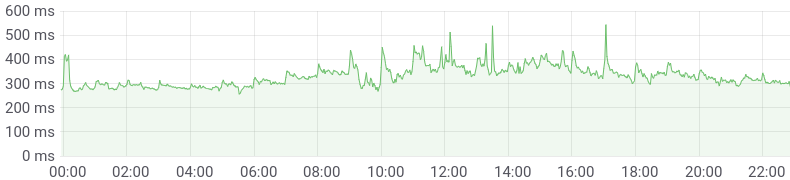
\includegraphics[scale=0.6]{timings.png}
	\caption{Среднее время обработки письма}
	\label{fig:03}
\end{figure}


\begin{figure}[h!]
	\center
	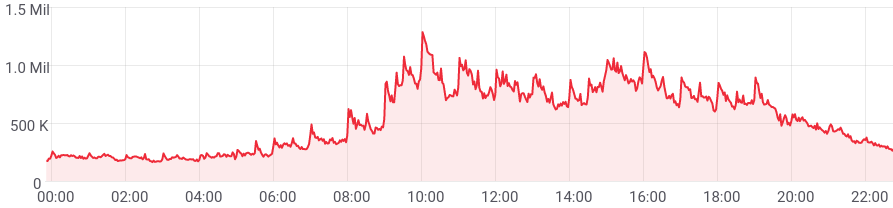
\includegraphics[scale=0.5]{processed_messages.png}
	\caption{Среднее количество запросов в минуту с одной из ферм}
	\label{fig:04}
\end{figure}

\subsubsection*{\it\,Обзор библиотек}

Since services require high performance, the C++ language (stl 17, grpc, boost) is chosen for writing it, as one of the most productive modern languages. For data analysis and training of the AST model, the Python 3 language and the utouch framework were used due to the high efficiency and the possibility of conducting parallel calculations, both on the CPU and on the GPU cores of the machine.

The fault tolerance of microservices is ensured by their deployment in the kubernetes (k8s) cluster, since if any pod falls for any reason, the requests are evenly balanced across the remaining live feeds, until the cluster independently returns to its previous state. Inside it, you can configure: automatic load balancing by constantly monitoring information about performance and resources used (autoscaling) and competent placement of hearths within the cluster by data centers (affinity).

\section{Conclusions}

This article presents the results obtained during the training of the model on real streaming data of users. Based on these data, we can conclude that the $FCNN$ model based on $Fast Text$ embeddings has the highest classification accuracy, compared to the methods of classical logistic regression and the $FCNN$ model based on a bag of words.


A high-performance fault-tolerant micro-service architecture is presented, which can withstand an average of more than $10^6$  requests per minute. At the same time, the degradation of a specific component, machine, or data center does not lead to complete inactivity of the application.

\begin{thebibliography}{99}
\bibitem{Makkar2021} 
Aaisha Makkar, Uttam Ghosh, Pradip Kumar Sharma.
2021. \emph{Artificial Intelligence and Edge Computing-enabled
	Web Spam Detection for Next Generation IoT
	Applications} // IEEE Sensors Journal

\bibitem{Taylor2020}
Taylor O.E., Ezekiel P.S.
2020. \emph{A Model to Detect Spam Email Using Support Vector Classifier and Random Forest Classifier} //
International Journal of Computer Science and Mathematical Theory

\bibitem{Garg2021}
Pranjul Garg, Nancy Girdhar.
2021. \emph{A systematic review on spam filtering techniques based on
natural language processing framework} // 2021 11th International Conference on Cloud Computing, Data Science \& Engineering (Confluence 2021)

\bibitem{Parmar2020}
Nandan Parmar, Ankita Sharma, Harshita Jain, Amol K. Kadam.
2020. \emph{Email Spam Detection using Naïve Bayes and Particle Swarm Optimization} // IJIRT

\bibitem{Mohammad2020}
Rami Mustafa A. Mohammad.
2020. \emph{A lifelong spam emails 	classification model} //
Applied Computing and Informatics
\end{thebibliography}



\end {document}
